\documentclass[11pt,landscape]{article}
\usepackage[margin=10mm]{geometry}
\usepackage{iftex}
\ifPDFTeX
  \usepackage[T2A]{fontenc}
  \usepackage[utf8]{inputenc}
  \usepackage[russian,english]{babel}
\else
  \usepackage{fontspec}
  \usepackage{polyglossia}
  \setdefaultlanguage{russian}
  \setotherlanguage{english}
  \setmainfont{DejaVu Serif}
  \setsansfont{DejaVu Sans}
  \setmonofont{DejaVu Sans Mono}
\fi
\usepackage{graphicx}
\usepackage{amsmath}
\usepackage{amssymb}
\usepackage{tikz}
\usetikzlibrary{arrows.meta, positioning, fit, backgrounds, calc, decorations.pathreplacing}
\pagestyle{empty}

\begin{document}

\noindent\makebox[\textwidth][c]{\Large GRLNet-StabhRec: общая концепция рекуррентной развертки}

\vspace{2mm}

\begin{center}
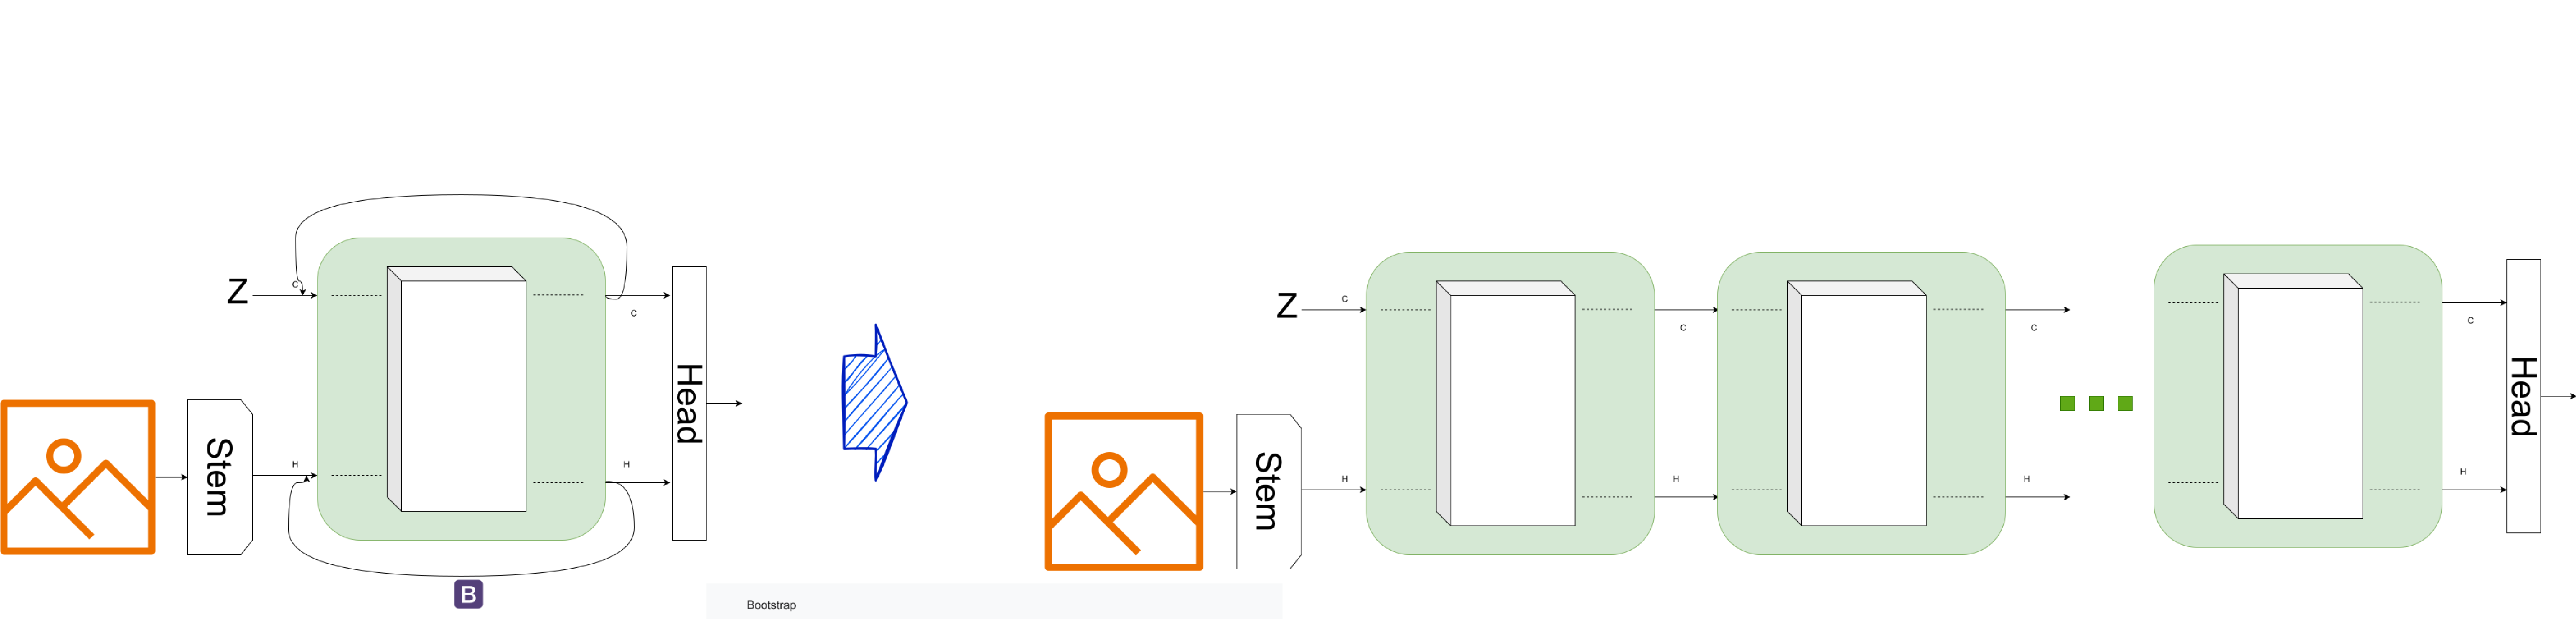
\includegraphics[width=\textwidth]{grlnet_stabhrec40_temporal_bottom.drawio.pdf}
\end{center}

\vspace{1mm}

\noindent\textbf{Общая идея.}
Однослойная модель \textit{GRLNet-StabhRec} не содержит 12 различных сверточных блоков по глубине. Вместо этого она использует один \textit{stem}, один блок инициализации скрытого состояния \textit{$h$-seed}, одну общую рекуррентную ячейку и одну основную классификационную голову. Рекуррентная ячейка применяется 12 раз подряд к скрытому состоянию фиксированного размера, поэтому эффективная глубина сети возникает за счет временной развертки, а не за счет стека разных слоев с независимыми параметрами.

\medskip

\noindent
На концептуальной диаграмме верхний поток помечен маленькой буквой $c$ и соответствует каналу памяти $C$. Обозначение $Z$ на входе указывает на нулевую начальную инициализацию этого канала перед началом рекуррентной развертки.

\medskip

\noindent
Если считать только уникальные trainable Conv/Linear-слои, то при инференсе модель содержит 9 слоев: 3 слоя в \textit{stem}, 1 слой в \textit{$h$-seed}, 3 сверточных слоя в рекуррентной ячейке и 2 линейных слоя в основной голове. Во время обучения дополнительно присутствует \textit{aux-head}, что дает еще 2 линейных слоя и увеличивает число уникальных trainable-слоев до 11.

\medskip

\noindent
Если же рассматривать сеть в полностью развернутом по времени виде и считать каждое применение общей ячейки как отдельный вычислительный этап, то эффективная глубина возрастает. При инференсе получаем:
\[
3 \; (\textit{stem}) + 1 \; (h\text{-seed}) + 12 \times 3 \; (\textit{cell}) + 2 \; (\textit{main head}) = 42
\]
\noindent
последовательных Conv/Linear-преобразования. Таким образом, \textit{GRLNet-StabhRec} можно интерпретировать как компактную архитектуру с небольшим числом уникальных параметризованных слоев, но с существенно большей эффективной глубиной в развернутом режиме.

\newpage

\noindent\makebox[\textwidth][c]{\Large GRLNet-StabhRec: single-layer recurrent architecture}

\vspace{2mm}

\resizebox{\textwidth}{!}{%
\begin{tikzpicture}[
    >=Latex,
    font=\small,
    io/.style={draw, rounded corners=3pt, very thick, align=center, inner sep=4pt, fill=green!7, minimum width=25mm, minimum height=11mm},
    block/.style={draw, rounded corners=3pt, very thick, align=center, inner sep=4pt, fill=blue!6, minimum width=31mm, minimum height=13mm},
    state/.style={draw, rounded corners=3pt, very thick, align=center, inner sep=4pt, fill=cyan!7, minimum width=26mm, minimum height=11mm},
    head/.style={draw, rounded corners=3pt, very thick, align=center, inner sep=4pt, fill=orange!10, minimum width=28mm, minimum height=11mm},
    op/.style={draw, rounded corners=2pt, thick, align=center, inner sep=3pt, fill=yellow!10, minimum width=21mm, minimum height=9mm},
    main/.style={->, very thick},
    hpath/.style={->, very thick, draw=teal!70!black},
    cpath/.style={->, very thick, draw=magenta!75!black},
    auxpath/.style={->, thick, dashed, draw=orange!80!black},
    note/.style={draw, rounded corners=2pt, align=left, inner sep=3pt, fill=white, text width=42mm}
]

% --------------------------------------------------------------------------
% Overall architecture
% --------------------------------------------------------------------------
\node[io, minimum width=22mm] (input) at (0.0,4.7) {Input image\\$3 \times 224 \times 224$};

\node[block, minimum width=36mm] (stem) at (3.9,4.7) {Stem\\ConvGNAct $5\times5$/2\\ConvGNAct $3\times3$\\MaxPool $3\times3$/2\\ConvGNAct $3\times3$\\$64 \times 56 \times 56$};

\node[block, minimum width=29mm] (seed) at (8.9,4.7) {$h$-seed\\Conv $64 \to 192$\\GroupNorm + SiLU\\$192 \times 56 \times 56$};

\node[state, minimum width=25mm] (init) at (12.8,4.7) {Initial state\\$h_0 = h_{\text{seed}}$\\$c_0 = 0$};

\node[block, minimum width=36mm, minimum height=18mm] (unroll) at (19.2,4.7) {Общая рекуррентная\\ячейка\\одни веса на всех шагах\\итерации $t=1,\dots,12$\\$(h_{t-1},c_{t-1}) \mapsto (h_t,c_t)$};

\draw[main] (input.east) -- (stem.west);
\draw[main] (stem.east) -- (seed.west);
\draw[main] (seed.east) -- (init.west);
\draw[main] (init.east) -- (unroll.west);

\draw[hpath] ($(unroll.east)+(0,3mm)$) .. controls +(18mm,0) and +(18mm,0) .. ($(unroll.east)+(0,-3mm)$);
\node[anchor=south, font=\scriptsize, text=teal!70!black, fill=white, inner sep=1pt] at ($(unroll.east)+(17mm,4mm)$) {$h_t \rightarrow h_{t+1}$};
\draw[cpath] ($(unroll.west)+(0,3mm)$) .. controls +(-16mm,0) and +(-16mm,0) .. ($(unroll.west)+(0,-3mm)$);
\node[anchor=north, font=\scriptsize, text=magenta!75!black, fill=white, inner sep=1pt] at ($(unroll.west)+(-14mm,-4mm)$) {$c_t \rightarrow c_{t+1}$};

\draw[decorate, decoration={brace, amplitude=5pt}] ($(unroll.south west)+(-2mm,-4mm)$) -- ($(unroll.south east)+(2mm,-4mm)$)
    node[midway, below=6pt] {\scriptsize рекуррентная развертка с фиксированным пространственным разрешением};

% Late readouts
\coordinate (tap10) at ($(unroll.east)+(0,14mm)$);
\coordinate (tap11) at ($(unroll.east)+(0,0mm)$);
\coordinate (tap12) at ($(unroll.east)+(0,-14mm)$);

\node[op, minimum width=24mm] (ro10) at (25.6,6.1) {Readout\\step 10\\$[GAP(h_{10}); GAP(c_{10})]$};
\node[op, minimum width=24mm] (ro11) at (25.6,4.7) {Readout\\step 11\\$[GAP(h_{11}); GAP(c_{11})]$};
\node[op, minimum width=24mm] (ro12) at (25.6,3.3) {Readout\\step 12\\$[GAP(h_{12}); GAP(c_{12})]$};

\draw[hpath] (tap10) -- (ro10.west);
\draw[hpath] (tap11) -- (ro11.west);
\draw[hpath] (tap12) -- (ro12.west);

\node[head, minimum width=26mm] (auxhead) at (31.0,5.7) {Aux head\\LayerNorm\\Linear $384\to256$\\GELU, Dropout\\Linear $\to K$};
\node[head, minimum width=26mm] (mainhead) at (31.0,3.3) {Main head\\LayerNorm\\Linear $384\to512$\\GELU, Dropout\\Linear $\to K$};

\draw[auxpath] (ro10.east) -- (auxhead.west);
\draw[auxpath] (ro11.east) -- (auxhead.west);
\draw[main] (ro12.east) -- (mainhead.west);

\node[io, minimum width=21mm] (auxlogits) at (35.4,5.7) {Aux logits\\$y'_{10}, y'_{11}$};
\node[io, minimum width=21mm] (mainlogits) at (35.4,3.3) {Main logits\\$y$};

\draw[auxpath] (auxhead.east) -- (auxlogits.west);
\draw[main] (mainhead.east) -- (mainlogits.west);

\node[note, text width=48mm] (n1) at (35.1,0.45) {
\textbf{Поздняя супервизия.}\\
Блок чтения подключается только к последним трем шагам.
Вспомогательная голова используется для шагов 10 и 11 во время обучения;
основная голова использует шаг 12 и сохраняется для инференса.
};

\begin{scope}[on background layer]
    \node[draw, rounded corners=4pt, thick, fit=(input)(stem)(seed)(init)(unroll)(ro10)(ro11)(ro12)(auxhead)(mainhead)(auxlogits)(mainlogits)(n1), inner sep=6pt, fill=gray!3] {};
\end{scope}

\end{tikzpicture}
}

\vspace{4mm}

\noindent\textbf{Текстовое описание общей схемы.}
Входное изображение размера $3\times224\times224$ сначала обрабатывается блоком \textit{stem}, который уменьшает пространственное разрешение до $56\times56$ и формирует карту признаков размера $64\times56\times56$. Затем блок $h$-seed отображает этот тензор в скрытое рекуррентное пространство, создавая начальное состояние $h_0\in\mathbb{R}^{192\times56\times56}$, тогда как состояние памяти инициализируется как $c_0=0$.

\medskip

\noindent
Ядром модели является одна общая рекуррентная ячейка, применяемая в течение 12 последовательных шагов. Одни и те же параметры ячейки используются на каждом шаге, поэтому сеть увеличивает эффективную глубину за счет итеративного уточнения, а не за счет стека различных слоев. В течение всей рекуррентной развертки и скрытое состояние, и состояние памяти остаются на одной и той же пространственной сетке.

\medskip

\noindent
Предсказания снимаются не с каждого рекуррентного шага. Вместо этого блоки readout подключаются только к последним трем шагам, а именно к шагам 10, 11 и 12. На каждом из этих шагов модель выполняет глобальный average pooling как для $h_t$, так и для $c_t$, конкатенирует полученные векторы и использует итоговое представление как вход классификатора.

\medskip

\noindent
Финальная предиктовая голова работает с readout шага 12 и формирует logits для инференса. Во время обучения дополнительная auxiliary-head применяется также к readout шагов 10 и 11, обеспечивая позднюю дополнительную супервизию. Таким образом, при инференсе используется только последнее рекуррентное состояние, тогда как обучение получает дополнительный сигнал ошибки на двух предшествующих поздних шагах.

\vspace{5mm}

\noindent\textbf{Ключевые элементы рецепта обучения.}
Для однослойной модели на \textit{ImageNet-1K} использовался оптимизатор \texttt{SGD + Nesterov momentum} с линейным warmup на первых эпохах и последующим \textit{cosine decay}. Основной loss строился как \texttt{CrossEntropy} с \texttt{label smoothing}, а к шагам 10 и 11 дополнительно подключался auxiliary-loss, так что обучение происходило не только по последнему шагу развертки, но и по двум поздним промежуточным readout.

\medskip

\noindent
Существенной частью рецепта является \textit{MixUp}: на стадии обучения входные батчи с некоторой вероятностью заменяются линейной смесью двух изображений, а loss считается как та же выпуклая комбинация двух target-функций. Поэтому train-метрики вычисляются в более жестком режиме, чем clean validation. Кроме того, после каждого шага оптимизации обновляется \textit{EMA}-копия весов модели; именно эта сглаженная по времени версия затем используется для валидации, выбора лучших checkpoint и итогового инференса. Это важно учитывать при интерпретации различий между train- и val-кривыми.

\medskip

\noindent
На уровне вычислительного recipe обучение выполнялось в mixed-precision режиме с дополнительным \textit{gradient clipping}; для ускорения использовались \texttt{channels\_last} и аппаратные оптимизации уровня \textit{A100}. Эти детали не меняют формулу модели, но входят в фактический тренировочный протокол и поэтому важны для корректного воспроизведения результатов.

\vspace{5mm}

\noindent\textbf{Отдельная схема Stem.}

\vspace{2mm}

\begin{center}
\begin{tikzpicture}[
    >=Latex,
    font=\small,
    stemio/.style={draw, rounded corners=3pt, very thick, align=center, inner sep=4pt, fill=green!7, minimum width=23mm, minimum height=10mm},
    stemblock/.style={draw, rounded corners=3pt, very thick, align=center, inner sep=3pt, fill=blue!6, minimum width=24mm, minimum height=12mm, text width=22mm},
    stemmain/.style={->, very thick}
]

\node[stemio] (sin) at (0,0) {Вход\\$3\times224\times224$};

\node[stemblock] (s1) at (3.4,0) {Conv\\GroupNorm\\SiLU\\$5\times5$, stride 2\\$3 \to 64$\\$64\times112\times112$};
\node[stemblock] (s2) at (6.8,0) {Conv\\GroupNorm\\SiLU\\$3\times3$, stride 1\\$64 \to 64$\\$64\times112\times112$};
\node[stemblock] (s3) at (10.2,0) {MaxPool\\$3\times3$, stride 2\\каналы без изм.\\$64\times56\times56$};
\node[stemblock] (s4) at (13.6,0) {Conv\\GroupNorm\\SiLU\\$3\times3$, stride 1\\$64 \to 64$\\$64\times56\times56$};

\node[stemio] (sout) at (16.9,0) {Выход stem\\$64\times56\times56$};

\draw[stemmain] (sin.east) -- (s1.west);
\draw[stemmain] (s1.east) -- (s2.west);
\draw[stemmain] (s2.east) -- (s3.west);
\draw[stemmain] (s3.east) -- (s4.west);
\draw[stemmain] (s4.east) -- (sout.west);

\end{tikzpicture}
\end{center}

\vspace{1mm}

\noindent\textbf{Краткое описание блока Stem.}
Первый сверточный слой с ядром $5\times5$ и шагом 2 выполняет начальное извлечение локальных признаков и одновременно уменьшает пространственное разрешение входа. Второй сверточный слой $3\times3$ уточняет полученные низкоуровневые признаки без изменения числа каналов и пространственного масштаба. Затем операция max-pooling дополнительно уменьшает разрешение, сохраняя наиболее выраженные локальные ответы. Последний сверточный слой $3\times3$ формирует итоговое представление блока \textit{stem} размера $64\times56\times56$, которое затем подается на вход блока $h$-seed для инициализации рекуррентного скрытого состояния.

\newpage

\noindent\textbf{Отдельная схема рекуррентной ячейки.}

\vspace{2mm}

\begin{center}
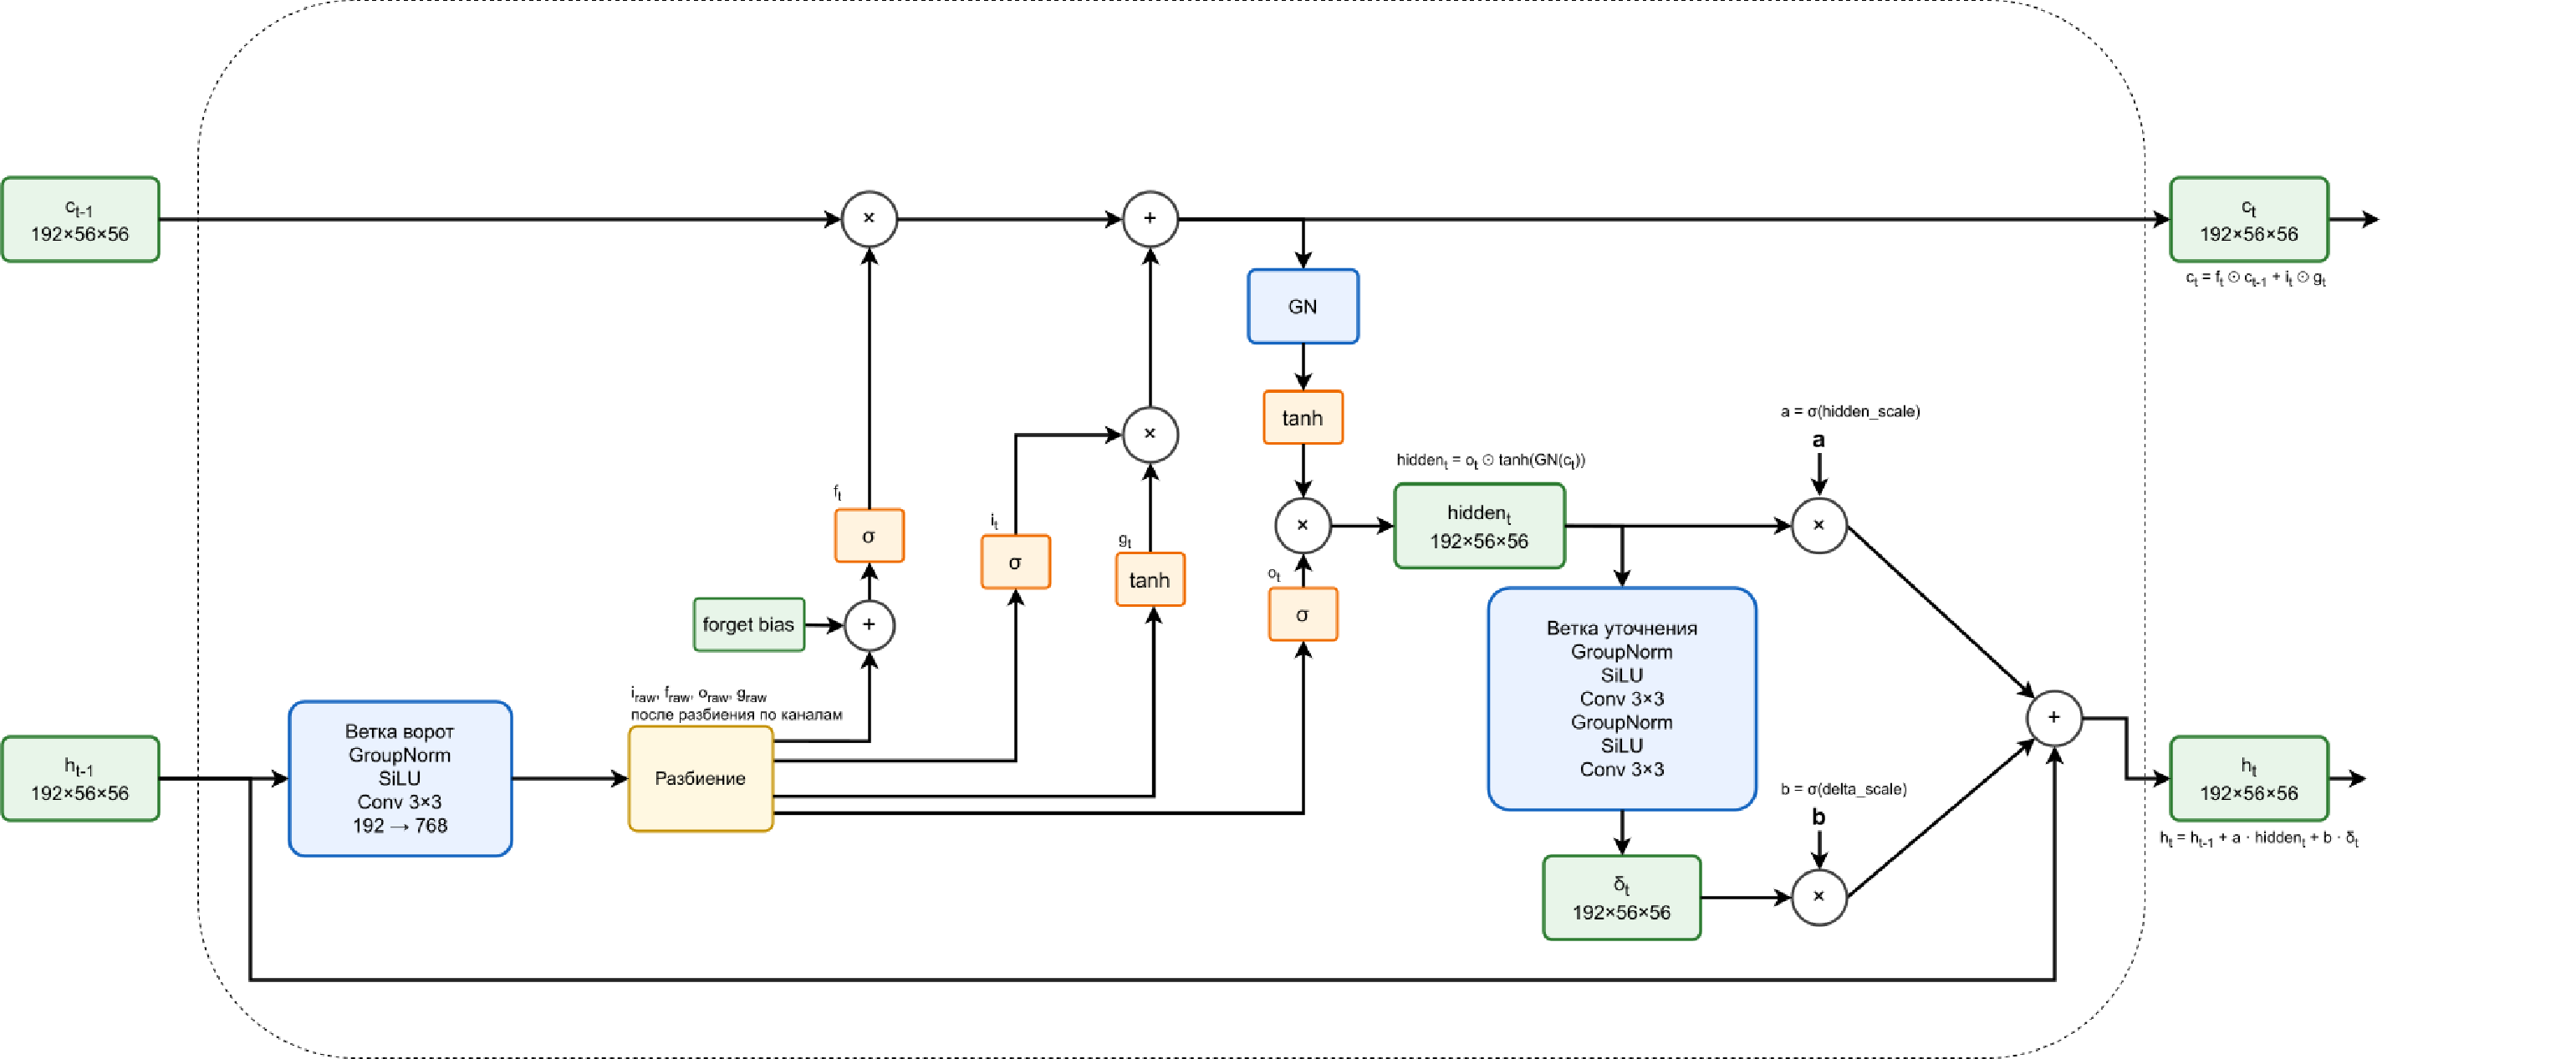
\includegraphics[width=\textwidth]{grlnet_stabhrec40.drawio.pdf}
\end{center}

\vspace{1mm}

\noindent\textbf{Подробное описание этапов обработки в рекуррентной ячейке.}
На вход ячейки поступают два состояния предыдущего шага: скрытое состояние $h_{t-1}$ и состояние памяти $c_{t-1}$. Сначала из $h_{t-1}$ через ветку \textit{gate branch} последовательно вычисляются нормализованные и нелинейно преобразованные признаки, после чего свертка формирует тензор из четырех групп каналов. Этот тензор разбивается на сырые карты $i_{raw}$, $f_{raw}$, $o_{raw}$ и $g_{raw}$, соответствующие входным воротам, воротам забывания, выходным воротам и кандидату обновления памяти.

\medskip

\noindent
Далее к ветви забывания добавляется константный \textit{forget bias}, после чего применяются нелинейности: сигмоида для $i_t$, $f_t$ и $o_t$, а гиперболический тангенс для $g_t$. Состояние памяти обновляется по LSTM-подобному правилу
\[
c_t = f_t \odot c_{t-1} + i_t \odot g_t,
\]
где одна часть старой памяти сохраняется через $f_t$, а новая информация записывается через $i_t$ и $g_t$.

\medskip

\noindent
После этого новое состояние памяти $c_t$ нормализуется, проходит через функцию $\tanh$ и затем поэлементно умножается на выходные ворота $o_t$. Так формируется основной кандидат обновления скрытого состояния
\[
hidden_t = o_t \odot \tanh(GN(c_t)).
\]
Этот сигнал отражает основной результат текущего рекуррентного шага.

\medskip

\noindent
Затем $hidden_t$ подается в дополнительную ветку \textit{delta / refine}, состоящую из двух последовательных блоков \textit{GroupNorm $\rightarrow$ SiLU $\rightarrow$ Conv}. Эта ветка вычисляет корректирующую добавку $\delta_t$, предназначенную для более тонкого нелинейного уточнения скрытого состояния. Таким образом, основная ветвь задает базовое gated-обновление, а refine-ветка формирует дополнительную поправку к нему.

\medskip

\noindent
На последнем этапе старое скрытое состояние $h_{t-1}$ передается по residual-связи напрямую к выходу ячейки. К нему добавляются два новых вклада: основной сигнал $hidden_t$ и корректирующий сигнал $\delta_t$, каждый со своим обучаемым скалярным коэффициентом:
\[
h_t = h_{t-1} + a \cdot hidden_t + b \cdot \delta_t,
\qquad
a=\sigma(hidden\_scale), \quad b=\sigma(delta\_scale).
\]
Коэффициенты $a$ и $b$ являются обучаемыми глобальными весами, которые регулируют, насколько сильно в итоговое скрытое состояние должны входить основной gated-update и refine-поправка. В результате выходами ячейки становятся обновленные состояния $c_t$ и $h_t$, сохраняющие ту же пространственную структуру, что и на входе.

\vspace{4mm}

\noindent\textbf{Численная проверка вклада компонентов ячейки.}
Для проверки того, что ветви ячейки не являются декоративными, была проведена inference-only диагностика на первых 256 изображениях из \textit{ImageNet-1K val} с использованием лучшего EMA-checkpoint однослойной модели (\texttt{epoch 49}, \texttt{best val top-1 = 67.91\%}). На этом подмножестве базовая модель дает \texttt{67.58\%} \textit{top-1}. Затем из forward-pass поочередно удалялись отдельные компоненты ячейки.

\medskip

\begin{center}
\small
\begin{tabular}{|l|c|c|l|}
\hline
\textbf{Вариант} & \textbf{Top-1, \%} & \textbf{$\Delta$ к baseline, п.п.} & \textbf{Интерпретация} \\
\hline
Базовая модель & 67.58 & 0.00 & Все ветви активны \\
\hline
Без $C$ в readout & 4.69 & -62.89 & $C$ несет критическую информацию в классификатор \\
\hline
Без переноса памяти $f_t \odot c_{t-1}$ & 25.00 & -42.58 & Канал $C$ работает как память, а не только как градиентный обход \\
\hline
Без вклада $a \cdot hidden_t$ & 64.06 & -3.52 & Основной gated-update информативен, хотя не доминирует \\
\hline
Без вклада $b \cdot \delta_t$ & 3.13 & -64.45 & Refine-ветка критична для качества \\
\hline
Занулены conv-веса в gate/refine & 0.39 & -67.19 & Один residual-путь по $H$ почти не работает без рекуррентных сверток \\
\hline
Без residual-связи по $h_{t-1}$ & 0.00 & -67.58 & Residual-ветвь необходима для устойчивого накопления состояния \\
\hline
\end{tabular}
\normalsize
\end{center}

\medskip

\noindent
Эти абляции показывают, что в текущей версии архитектуры канал $C$ уже нельзя интерпретировать только как вспомогательный путь для протечки градиента. Напротив, он выполняет две содержательные функции: во-первых, аккумулирует gated-memory через член $f_t \odot c_{t-1}$; во-вторых, напрямую участвует в readout, и удаление pooled-$C$ из классификатора почти разрушает качество. Таким образом, residual-связь по $H$ действительно берет на себя роль стабильной магистрали распространения сигнала, а $C$ смещается в сторону памяти и пространственно согласованного накопления признаков.

\medskip

\noindent
Параметры смешивания после обучения принимают значения $a=\sigma(hidden\_scale)=0.0674$ и $b=\sigma(delta\_scale)=0.0255$. Несмотря на то, что $b < a$, фактический вклад refine-ветки оказывается выше из-за большой нормы $\delta_t$. На шагах 1, 6 и 12 средние RMS-вклады равны: для $a \cdot hidden_t$ --- \texttt{0.0115 / 0.0074 / 0.0051}, а для $b \cdot \delta_t$ --- \texttt{0.0321 / 0.0301 / 0.0296}. Это означает, что $\delta$-ветка не просто слегка корректирует hidden-update, а фактически выступает главным механизмом уточнения состояния на поздних шагах. При этом вклад $a \cdot hidden_t$ остается ненулевым и его удаление все же снижает top-1 на \texttt{3.52} п.п., поэтому базовый gated-update также информативен.

\medskip

\noindent
Отдельная абляция с занулением всех рекуррентных сверток внутри ячейки --- как в gate-ветке, так и в refine-ветке --- дополнительно показывает, что residual-связь по $H$ не шунтирует рекуррентную обработку. В этом режиме сеть фактически сводится к \textit{stem} $\rightarrow$ \textit{h\_seed} $\rightarrow$ многократному тождественному переносу $H$ $\rightarrow$ \textit{readout/head}, однако top-1 падает до \texttt{0.39\%}. Следовательно, высокая точность базовой модели не может объясняться одним лишь глубоким residual-путем: рекуррентные сверточные преобразования внутри ячейки действительно выполняют основную содержательную работу.

\medskip

\noindent
Важно, однако, что приведенная абляция относится только к стадии инференса: обученная модель тестируется с искусственно отключенным членом $a \cdot hidden_t$. Поэтому эти числа не исключают, что данный член играет более существенную роль именно во время оптимизации, стабилизируя ранние шаги обучения и помогая сформировать ту динамику, в которой refine-ветка $\delta_t$ затем берет на себя основную часть позднего уточнения.

\vspace{4mm}

\noindent\textbf{Численная диагностика протечки градиента.}
Чтобы уточнить роль каналов $H$ и $C$ в текущей архитектуре, была дополнительно измерена обратная протечка градиента через рекуррентную развертку. Для этого на первых 128 изображениях из \textit{ImageNet-1K val} вычислялся backward по loss, соответствующему финальной стадии обучения:
\[
\mathcal{L} = \mathcal{L}_{main} + 0.05 \cdot \mathcal{L}_{aux},
\]
где использовалась \texttt{CrossEntropyLoss} с \texttt{label smoothing = 0.05}, а auxiliary loss подключался к шагам 10 и 11 так же, как в основном рецепте обучения.

\medskip

\begin{center}
\small
\begin{tabular}{|l|c|c|c|}
\hline
\textbf{Величина} & \textbf{Шаг 1} & \textbf{Шаг 6} & \textbf{Шаг 12} \\
\hline
$\|\partial \mathcal{L} / \partial h_t\|_{RMS}$ & 0.001103 & 0.000368 & 0.000024 \\
\hline
$\|\partial \mathcal{L} / \partial c_t\|_{RMS}$ & 0.000089 & 0.000034 & 0.000106 \\
\hline
$\|\partial \mathcal{L} / \partial h_t\| / \|\partial \mathcal{L} / \partial c_t\|$ & 12.51 & 10.95 & 0.24 \\
\hline
\end{tabular}
\normalsize
\end{center}

\medskip

\noindent
Полученная картина показывает, что исходный тезис о канале $C$ как основном носителе глубокого градиента уже не соответствует новой архитектуре. На ранних и средних шагах рекуррентности градиент по каналу $H$ оказывается примерно в 11--13 раз сильнее, чем по каналу $C$, что хорошо согласуется с появлением прямой residual-связи
\[
h_t = h_{t-1} + a \cdot hidden_t + b \cdot \delta_t.
\]
Именно эта связь превращает $H$ в основную магистраль переноса градиента через глубокую развертку.

\medskip

\noindent
В то же время канал $C$ не становится декоративным. Во-первых, его градиент остается ненулевым на всех шагах. Во-вторых, на последнем шаге градиент по $C$ даже превосходит градиент по $H$, поскольку pooled-$C$ напрямую входит в readout и влияет на классификатор. Таким образом, в текущей модели $C$ естественнее интерпретировать не как главный обходной путь для градиента, а как memory-ветвь, которая аккумулирует gated-state, участвует в позднем readout и добавляет собственный обучающий сигнал в окрестности выходных шагов.

\end{document}
